\svnid{$Id$}

\section{Additive Schwarz methods}

\begin{intro}
  In this section, we study preconditioners, which are related to
  subspace decompositions of the space $V$ or its finite dimensional
  subspaces. We will develop the theory in an abstract way, but always
  keep the model problem~\eqref{eq:main:1} in mind when we do so. In
  particular, the subspaces chosen will be associated with either
  coarser mesh levels or with meshes on subdomains of $\Omega$.
  
  This section follows in part~\cite[Chapter 7]{BrennerScott02}.
\end{intro}

\subsection{The abstract framework}

\begin{intro}
  Let $V$ be a Hilbert space and let $a(.,.): V\times V$ be a
  symmetric and $V$-elliptic bilinear form. Let the set of auxiliary
  subspaces $\{V_j\}_{j=0,\dots,J}$ of $V$ be chosen such that
  \begin{gather*}
    V = \sum_{j=0}^J V_j,
  \end{gather*}
  but the sum is not required to be direct, that is, a vector $v\in V$
  may have several decompositions $v = \sum \alpha_j v_j$ with $v_j\in
  V_j$.
\end{intro}

\begin{lemma}
  If the form $a(.,.)$ is bounded and V-elliptic, then the weak
  formulation: find $u_j\in V_j$ such that
  \begin{gather}
    \label{eq:schwarz:1}
    a(u_j,v_j) = f(v_j),
    \quad\forall v_j\in V_j,
  \end{gather}
  has a unique solution for all $f\in V^*$.
\end{lemma}

\begin{proof}
  This lemma follows from the fact that boundedness and V-ellipticity
  transfer from $V$ to its subspaces.
\end{proof}

\begin{definition}
  \index{Pj@$P_j$}
  Let the operator $P_j: V \to V_j$ be defined as the solution
  operator $P_j u := u_j$ to the problem
  \begin{gather}
    \label{eq:schwarz:2}
    a(u_j,v_j) = a(u,v_j),\quad\forall v_j\in V_j.
  \end{gather}
  We call $P_j$ the $A$-orthogonal projection operator to
  $V_j$. Furthermore, we define the $V$-orthogonal projection operator
  \index{Pij@$\Pi_j$}
  $\Pi_j: V \to V_j$ as the solution operator $\Pi_j u := u_j$ to the problem
  \begin{gather}
    \label{eq:schwarz:3}
    \scal(u_j,v_j) = \scal(u,v_j),\quad\forall v_j\in V_j.
  \end{gather}
\end{definition}

\begin{definition}
  The additive Schwarz preconditioner for the operator $A$ associated
  with the symmetric, and $V$-elliptic bilinear form $a(.,.)$ with
  respect to the subspace decomposition $V_j$ is the mapping $B:
  V^*\to V$ such that
  \begin{gather}
    \label{eq:schwarz:4}
    B = \sum_{j=1}^J P_j A^{-1}.
  \end{gather}
\end{definition}

\begin{example}
  As a guiding example for the definition of these methods may serve
  the Jacobi iteration. To this end, let $V = \R^n$ with its Euclidean
  inner product $\scal(.,.)$. let $V_j = \operatorname{span}\{e_j\}$
  be the space spanned by the $j$th unit vector. Let $A$ be a
  symmetric, positive definite matrix and $a(u,v) = v^T A u$. Then,
  equation~\eqref{eq:schwarz:2} becomes
  \begin{gather*}
    e_j^T A u_j = e_j^T A u
    \quad \Leftrightarrow \quad
    P_j u = u_j = \frac1{a_{jj}}(A u)_j.
  \end{gather*}
  Since for this decomposition, the sum $V=\bigoplus V_j$ is direct,
  we obtain with $D=\operatorname{diag}(a_{11},\dots,a_{nn})$ the
  matrix representation
  \begin{gather*}
    (B u)_j = \frac1{a_{jj}}(A A^{-1} u)_j
    \quad \Leftrightarrow \quad
    B = D^{-1}.
  \end{gather*}
  From the Richardson method in operator
  form~\eqref{eq:richardson:11}, we obtain the iteration
  \begin{align*}
    u^{(k+1)} &= u^{(k)} - \omega_k \sum_{j=1}^J P_j \bigl(u^{(k)} -
    A^{-1}f\bigr)\\
    &= u^{(k)} - \omega_k D^{-1} \bigl(A u^{(k)} - f\bigr).
  \end{align*}
\end{example}

\begin{lemma}
  If $A$ is symmetric and positive definite, so is $B$ as defined
  in~\eqref{eq:schwarz:4}.
\end{lemma}

\begin{proof}
  \begin{todo}
    ...
  \end{todo}
\end{proof}

\begin{lemma}
  For $v\in V$ holds
  \begin{gather}
    \label{eq:schwarz:5}
    \scal(B^{-1}v,v) = \min_{v=\sum v_j} \sum_{j=1}^J a(v_j,v_j),
  \end{gather}
  where the minimum is taken over all possible decompositions of $v$
  into a sum of elements $v_j\in V_j$ with $j=1,\dots,J$.
\end{lemma}

\begin{proof}
  \begin{todo}
    ...
  \end{todo}
\end{proof}

%%%%%%%%%%%%%%%%%%%%%%%%%%%%%%%%%%%%%%%%%%%%%%%%%%%%%%%%%%%%%%%%%%%%%%
%%%%%%%%%%%%%%%%%%%%%%%%%%%%%%%%%%%%%%%%%%%%%%%%%%%%%%%%%%%%%%%%%%%%%%
\section{Two-level additive Schwarz preconditioner}
%%%%%%%%%%%%%%%%%%%%%%%%%%%%%%%%%%%%%%%%%%%%%%%%%%%%%%%%%%%%%%%%%%%%%%
%%%%%%%%%%%%%%%%%%%%%%%%%%%%%%%%%%%%%%%%%%%%%%%%%%%%%%%%%%%%%%%%%%%%%%

\begin{intro}
  This preconditioner is in the class of \putindex{domain
    decomposition} methods. The attribute \putindex{two-level} refers
  to the fact that we are considering finite element discretizations
  of~\eqref{eq:itintro:1} on two finite element meshes, the
  \putindex{fine mesh} $\T_h$ on which we desire to compute the
  solution, and the auxiliary \putindex{coarse mesh} $\T_H$. Both
  meshes cover the whole domain $\Omega$ (see
  Figure~\ref{fig:schwarz:ddmeshes}), and each cell of the coarse mesh
  is the union of cells of the fine mesh ($4\times 4$ fine cells in
  the figure).

  In addition to these two meshes, we introduce subdomains
  $\Omega_1,\Omega_2,\dots,\Omega_J$ of $\Omega$ such that each
  $\Omega_j$ is the union of cells in $\T_h$. We require that those
  subdomains overlap each other like the three examples in
  Figure~\ref{fig:schwarz:ddmeshes} on the right. A more precise
  definition of the required overlap follows.
\end{intro}

\begin{figure}[tp]
  \centering
  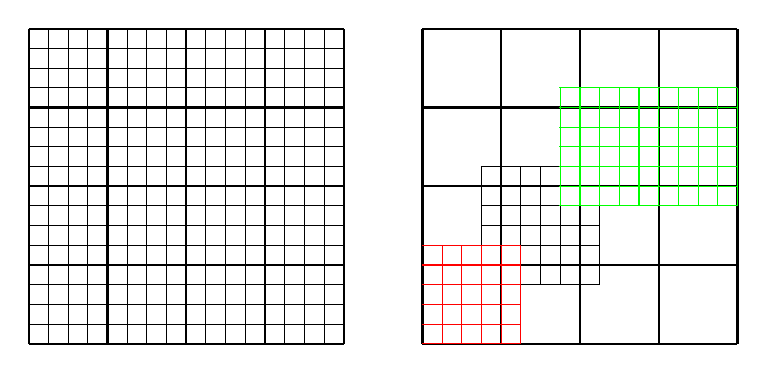
\begin{tikzpicture}
    \draw[step=.25cm] (-2,-2) grid (2,2);
    \draw[step=1cm,thick] (-2,-2) grid (2,2);
    \draw[step=1cm,thick] (3,-2) grid (7,2);
    \draw[step=.25cm] (3.74,-1.25) grid (5.25,0.25);
    \draw[step=.25cm,red] (3,-2) grid (4.25,-0.75);
    \draw[step=.25cm,green] (4.74,-0.25) grid (7,1.25);
  \end{tikzpicture}
  \caption{Fine mesh and coarse mesh (left) for overlapping domain
    decomposition. Examples for a subdomain decomposition on the
    right.}
  \label{fig:schwarz:ddmeshes}
\end{figure}

\begin{definition}
  A smooth \define{partition of unity} with respect to the subdomains
  $\Omega_1,\Omega_2,\dots,\Omega_J$ of $\Omega$ is a set of
  nonnegative functions $\{\phi_1,\dots,\phi_J\}\subset
  C^\infty(\overline\Omega)$ such that
  \begin{xalignat}2
    \label{eq:schwarz:6}
    \phi_j(x) &  = 0
    & \forall x & \in \Omega\setminus\Omega_j, \quad j=1,\dots,J
    \\
    \label{eq:schwarz:7}
    \sum_{j=1}^J \phi_j(x) &= 1
    & \forall x&\in\overline\Omega.
  \end{xalignat}
  Furthermore, we assume that there is a positive constant $\delta$,
  called \define{overlap}, such that for all $j=1,\dots,J$ there holds
  \begin{gather}
    \label{eq:schwarz:8}
    \norm{\nabla\phi j}_{L^\infty(\Omega)} \lesssim \frac 1\delta,
  \end{gather}
  where the implicit constant is independent of $h$, $\delta$ and $J$.
\end{definition}

\begin{note}
  The term overlap for $\delta$ is justified by the following
  consideration. Let $x \in \Omega_j$ be a point which is not in any
  other $\Omega_i$. Then, $\phi_j(x) = 1$. If~\eqref{eq:schwarz:8} is
  to hold, then it is necessary
  $\operatorname{dist}(x,\partial\Omega_J) \ge \delta$ (up to a
  constant, but this constant is already
  in~\eqref{eq:schwarz:8}). Thus, the points of distance less than
  $\delta$ from $\partial\Omega_j$ must be elements of another
  subdomain as well, which is then said to overlap with $\Omega_j$.
\end{note}

\begin{notation}
  The solution space of our problem is the space $V=V_h$ given by the
  finite element space on the mesh $\T_h$. Since the meshes are
  nested, the finite element space $V_0 \equiv V_H$ on the mesh $\T_H$ is a
  subspace of $V_h$. Additionally, we define finite element spaces on
  $\Omega_j$ by
  \begin{gather}
    \label{eq:schwarz:9}
    V_j = \bigl\{ v\in V_h \big| \forall x\in\Omega\setminus\Omega_j :
    v(x) =0\bigr\}.
  \end{gather}
\end{notation}

\begin{definition}
  Let the spaces $V_j$, $j=0,\dots,J$ be defined as above. Then, the
  \define{two-level Schwarz preconditioner} is defined as
  \begin{gather}
    \label{eq:schwarz:10}
    B_{\text{TLS}} = \sum_{j=0}^J P_j A^{-1} = \sum_{j=0}^J A_j^{-1} \Pi_j,
  \end{gather}
  where $P_j$ is defined according to~\eqref{eq:schwarz:2} and $A_j:
  V_j\to V_j^*$ by
  \begin{gather}
    \scal(A_j u_j, v_j)_V = a(u_j, v_j),\quad\forall u_j, v_j \in V_j.
  \end{gather}
\end{definition}

\begin{note}
  In order to simplify notation, we have assigned index zero to
  $V_H$. Thus, sums in future terms may either start at one, summing
  over subdomains, or at zero, summing over all subspaces.
\end{note}

\begin{lemma}
  There holds
  \begin{gather}
    \label{eq:schwarz:11}
    V_h = \sum_{j=1}^J V_j.
  \end{gather}
\end{lemma}

\begin{proof}
  Let $I_h: C(\overline\Omega) \to V_h$ be the interpolation operator
  of the finite element space. Then, for any given $v\in V_h$ define
  $v_j = I_h(\phi_j v)$, where $\phi_j$ is the function associated to
  $\Omega_j$ of a partition of unity for $\Omega_1,\dots,\Omega_J$.
  
  By definition of $\phi_j$, there holds $\phi_j v = 0$ on
  $\Omega\setminus\Omega_j$. Furthermore, we assumed that a mesh cell
  of $\T_h$ is either completely in $\Omega_j$ or completely in its
  complement. Since nodal values of a cell are located in the cell
  itself, this implies that $I_h (\phi_j v) = 0$ on
  $\Omega\setminus\Omega_j$. Therefore, $I_h (\phi_j v) \in V_j$.
  
  On the other hand, we use the linearity of the interpolation
  operator to obtain
  \begin{gather*}
    \sum_{j=1}^J v_j = \sum_{j=1}^J I_h(\phi_j v)
    = I_h\left(v\sum_{j=1}^J \phi_h\right)
    = I_h v = v,
  \end{gather*}
  thus, the $v_j$ are indeed a decomposition of $v$. Since $v\in V_h$
  was chosen arbitrarily, the lemma is proven.
\end{proof}

\begin{intro}
  The following lemmas serve to verify the assumptions of the abstract
  Theorem~\ref{???}.
\end{intro}

\begin{lemma}[Stable decomposition]
  \label{lemma:schwarz:stable-decomposition}
  Let $v_j\in V_j$ for $j=0,\dots,J$ be a composition of $v\in V_h$
  such that
  \begin{gather*}
    v=\sum_{j=0}^J v_j.
  \end{gather*}
  Then,
  \begin{gather}
    \label{eq:schwarz:12}
    a(v,v) \lesssim \sum_{j=0}^J a(v_j, v_j).
  \end{gather}
\end{lemma}

\begin{proof}
  \begin{todo}
    p. 187 f.
  \end{todo}
\end{proof}

\begin{lemma}
  For each $v\in V_h$ there exists a decomposition $v=\sum_{j=0}^J
  v_j$ with $v_j\in V_j$, such that
  \begin{gather}
    \label{eq:schwarz:13}
    \sum_{j=0}^J a(v_j, v_j)
    \lesssim \left(1+\frac H\delta\right)^2 a(v,v).
  \end{gather}
\end{lemma}

\begin{proof}
  \begin{todo}
    p. 189 f.
  \end{todo}
\end{proof}

\begin{theorem}
  \label{theorem:schwarz:two-level-convergence}
  Under the assumptions made so far in this section, there holds
  \begin{gather}
    \label{eq:schwarz:14}
    \kappa(B_{\text{TLS}} A_h)
    = \frac{\lambda(B_{\text{TLS}}, A_h)}{\Lambda(B_{\text{TLS}},
      A_h)}
    \lesssim \left(1+\frac H\delta\right)^2,
  \end{gather}
  where the implicit constant is independent of $h$, $\delta$, $H$, and $J$.
\end{theorem}

\begin{proof}
  \begin{todo}
    ...
  \end{todo}
\end{proof}

\begin{remark}
  \begin{todo}
    \begin{itemize}
    \item Size of overlap vs. numerical effort
    \item Size of overlap vs. coarse grid size
    \item Size of coarse grid and subdomains vs. speed
    \end{itemize}
  \end{todo}
\end{remark}

%%% Local Variables: 
%%% mode: latex
%%% TeX-master: "main"
%%% End: 
